\documentclass{article}
\usepackage[utf8]{inputenc}
\usepackage{amsmath}
\usepackage{mathtools}
\usepackage{bm}
\usepackage{graphicx}
\usepackage{float}
\title{COL352: Assignment 2}
\author{Sachin 2019CS10722 \\
        Saurabh Verma 2019CS50129\\
        Sriram Verma}
\date{March, 2022}

\begin{document}

\maketitle


\section{Question 1}
\textbf{We say that a context-free grammar G is self-referential if for some non-terminal symbol $X$ we have $X \to^* \alpha X \beta$, where $\alpha, \beta \neq \varepsilon$. Show that a CFG that is not self-referential is regular.}
\\
\textbf{Proof:}
Suppose our grammar G has has N symbols
$X_1,X_2....,X_N$ and for each pair i,j there exist strings $\alpha,\beta$ such that $X_i \implies \alpha X_j \beta$.\\
\textbf{Proof by induction(on number of non terminal symbols)}:\\
\textbf{(Base Step:(N=1)}Let G has only one n non terminal symbol X.Hence language is in the form $X \rightarrow aX $ or $X \rightarrow Xb $  a Finite state Language.Hence regular.\\
\textbf{Induction Hypothesis:(N<n)}Suppose grammar that is not self referential with less than n non terminal symbols is regular.\\
\textbf{Induction Step:(N=n)}
Let  G has n non terminal symbols $X_1,X_2....,X_n$.Let for some particular i,j,there doesnt exist strings $\alpha,\beta$ such that $X_j \implies \alpha X_i \beta$.Let L be language generated by this grammar G.Lets remove rule $X_j \implies \alpha$ from grammar G and create a new terminal symbol c such that $X_j \implies c$.Now this newly created grammar be $G_1$ and language generated from this grammar be $L_1$.From hypothesis,$L_1$ is regular and sets formed from $X_j \implies c$ is finite too.So,L is a finite state language.Hence L is regular.



\pagebreak

\section{Question 2}
\textbf{Prove that the class of context-free languages is closed under intersection with regular languages. That is, prove that if \boldsymbol{$L_1$} is a context-free language and \boldsymbol{$L_2$} is a regular language, then \boldsymbol{$L_1 \cap L_2$}
is a context-free language. Do this by starting with a DFA}\\
\newline
Let us suppose there is a CFL L and a regular langauage R. The pushdown automata that accepts L be P=$(S_1,\Sigma,\Gamma,\delta_1,s_1,F_1)$ and the DFA accepting R be D=$(S_2,\Sigma,\delta_2,s_2,F_2)$. Now we have to show that the language $L\cap R$ is CFL. To show this it is enough to provide a PDA that accepts it. So we will construct such a PDA to prove that  $L\cap R$ is CFL. \\
\textbf{To Prove:} $L\cap R$ is CFL. \\
\textbf{Proof:} We will the above hypothesis by construction. The main idea behind the construction of the PDA is that we will run both the original PDA P for L and the DFA D in parallel on the input string and will only accept when the we reach an accepting state both in P and D. The construction of the PDA is described below:\\
\textbf{Construction:} Let the PDA which accepts $L\cap R$ be M=$(S,\Sigma,\Gamma,\delta,(s_1,s_2),F)$. Here S is $S_1 * S_2$ and F is $F_1 *F_2$. The transition function $\delta$ is described as follow: \\
For all the transitions $((p_1,a,\alpha),(p_2,\beta)) \in \delta_1$  and $(q_1,a,q_2) \in \delta_2$ add the transition $(((p_1,q_1),a,\alpha),((p_2,q_2),\beta))$ in $\delta$.\\
Also, for all the transitions $((p_1,\epsilon,\alpha),(p_2,\beta)) \in \delta_1$  and $\forall q \in S_2$ add the transition $(((p_1,q),a,\alpha),((p_2,q),\beta))$ in $\delta$.\\
Here $p_1,p_2 \in S_1$  $q_1,q_2 \in S_2$  $a \in \Sigma$  $\alpha , \beta \in \Gamma$\\
The accepting condition is that the final state reached after reading the input must belong to F.\\
Now our claim is that PDA M exactly recognises every string that is in $L\cap R$. \\
\textbf{Claim:} The PDA M constructed above exactly recognises strings in $L\cap R$. \\
\textbf{Proof:} We will have to show two things first that every string in $L\cap R$ is accepted by M. Lets prove this. Choose any string w$\in L\cap R$. Then its run on the DFA D would be something like $s_2,q1......q_k$ where $q_k \in F_2$, also w would take the PDA M from start configuration($s_1$) to an accepting configuration($q_{k^{'}}$) in some steps. By the way we have constructed the PDA M the computions of M and D will happen in parallel. So (s1,s2) is the start configuration of the PDA. First state in the tuple denotes the state that would have been in the PDA P and second state denotes the state that would have been in the DFA D after reading input upto some point. So when the PDA gets to wun on w. It would take M from from (s1,s2) to $(q_k,q_{k^{'}})$. Now this is an accepting configuration in M by the way we defined F$(F_1 * F_2)$. So all the string  w$\in L\cap R$ are accepted by M.\\
Also we have to prove that all the strings say w that are accepted by M should also be present in $ L\cap R$. We will accept w if it takes PDA M from $(s_1,s_2)$ to $(q_1,q_2)$ , $q_1 \in F_1$ and $q_2 \in F_2$. Also we have showed that M is parallely running P and D where first state in the tuple means the state reached in P and second state means the state reached in D after reading the input uptill that point. So after reading  w if the M is in state $(q_1,q_2)$, it would mean that after reading w P would have been in $q_1$ and D would be in $q_2$. $q_1 \in F_1$, so $w \in L$ also $q_2 \in F_2$ so $w \in R$ which implies $w \in L \cap R$.\\
\newline
Thus we have successfully constructed a PDA M which accepts $L \cap M$. Thus CFL's are closed under intersection with regular languages. Hence proved. \\
\pagebreak


\section{Question 3}
\textbf{Given two languages $L, L'$, denote by $$L||L' := \{x_1y_1x_2y_2 \dots x_ny_n \mid x_1x_2 \dots x_n \in L, y_1y_2\dots y_n \in L'\}$$ Show that if \boldsymbol{$L$} is a CFL and $L'$ is regular, then \boldsymbol{$L || L'$} is a CFL by constructing a PDA for \boldsymbol{$L || L'$}. Is \boldsymbol{$L || L'$} a CFL if both \boldsymbol{$L$} and \boldsymbol{$L'$} are CFLs? Justify your answer.}\\
\newline 
For the first part we have to show that T=$L||L'$ is a CFL if L is CFL and $L'$ is regular. Since L is CFL we are given a PDA P=$(S_1,\Sigma,\Gamma,\delta_1,s_1,F_1)$ which recognizes it. Also we have a DFA D=$(S_2,\Sigma,\delta_2,s_2,F_2)$ which recognises $L'$. These are the things given to us.\\
\textbf{To Prove:} T is CFL.\\
\textbf{Proof Idea:} To show that T is CFL we would have to construct a PDA say R which accepts it. Now the main idea behind the working of this machine is that after reading alphabet of the input tape it would first check whether the position if odd or even (this can be done with an extra variable in the state) If the position is even then production rules of PDA P apply or else the transition rules of D apply. In the transitions we also have to update the position counter which tell us whether we are at odd or even location. So basically we are running PDA P on odd position and DFA D on even positions. The final accepting condition would be that position reached be even and states in both PDA P and DFA D are final. The specific construction of R is given as follows.\\
\textbf{Construction:} R=$(S,\Sigma,\Gamma,\delta,s,F)$. Here S is  $\{0,1\}*S_1 * S_2$ , F= $\{1\}*F_1 * F_2$. The start state s=$(1,s_1,s_2)$ The transition function $\delta$ is described as below\\
$\delta((1,p_1 ,q_1),a,\alpha)$ would contain $((0,p_2,q_1),\beta)$ if $\delta_1(p_1,a,\alpha)$ contained $(p_2,\beta)$.\\
$\delta((0,p_1 ,q_1),a,\alpha)$ would contain $((1,p_1,q_2),\alpha)$ if $\delta_2(q_1,a)$=$\{q_2\}$.\\
Here $p_1,p_2 \in S_1$  $q_1,q_2 \in S_2$  $a \in \Sigma$  $\alpha , \beta \in \Gamma$\\
The accepting condition is that the final state reached after reading the input must belong to F.\\
Now our claim is that PDA R exactly recognises every string that belongs to T. \\
\textbf{Claim:} R recognises the language T.\\
\textbf{Proof:} We have to show two things first that any string accepted by R belongs to T and every string belonging to T is accepted by R. \\
Let us consider any string $w $ and $w'$ $|w| = |w'|= n$. $t=w||w'$. Let the run of P be $(q_1,\epsilon)$ , $(q_2,\alpha_2) , (q_3,\alpha_3) .....(q_{n+1} ,\alpha_{n+1} )$ for w and the run of D on $w'$ be $p_1 , p_2 , q_3 ,.....p_{n+1} $. $q_1 = s_1$ and $q_2 =s_2$. Now what would be the run of $w || w'$ on R ? Start configuration of R would be $((1,q_1,p_1), \epsilon)$. Now the way we defined our transition function on odd positions it follows the the transition rules of P (and only second variable of the state tuple i.e. state of P would be modified)  and on even position rules of D (and only third variable of the state tuple i.e. state of D would be modified). We also know rules of D not make any changes in the stack. Thus after reading $2*i | i> 0$  length of input of t the configuration that R would be in is $((1,q_{i+1},p_{i+1}),\alpha_{i+1})$  and after reading $(2*i+1) |  i \geq 0$ configuration would be $((0,q_{i+1},p_{i}),\alpha_{i+1})$. Now when all the input is read i=n so the configuration that R would be in is $((1,q_{n+1},p_{n+1}),\alpha_{n+1})$.\\
If $w \in L$ then $q_{n+1} \in F_1$ and   $w' \in L'$ then $p_{n+1} \in F_2$. So when t=$w|| w'$ run on R final state $(1,q_{n+1},p_{n+1}) \in F$. So t is accepted. So every string in T is recognised by R. Now lets prove the other way.\\ 
Suppose R accepts a string t so final state $(1,q_{n+1},p_{n+1}) \in F$ which would mean $q_{n+1} \in F_1 \rightarrow  w \in L$ and $p_{n+1} \in F_2 \rightarrow w' \in L'$. Thus t=$w || w'$, $t \in T$. \\
Thus we have show that any string accepted by R belongs to T and every string belonging to T is accepted by R. So our claim that R recognizes T is true. \\
\newline
Since we have constructed a PDA R for the language T=$L || L'$ , we have sucessfully proved that T is indeed a CFL.
\\
\newline
Now let us see the second part of the question. Is $L||L'$ a CFL if both L and $L'$ are
CFLs? We will show that $L|| L'$ is not a CFL if L and $L'$ are CFls. \\
\textbf{To Prove:} $L|| L'$ is not a CFL if L and $L'$ are CFLs. \\
\textbf{Proof:} Giving a counter example will show that its not the case. Let us take two context free language and then we will show that $L || L'$ is not a CFL. L=$\{a^nb^n \ | \ n \geq 0\}$ . CFG for L is G=$(\{S\},\{a,b\},\{S \rightarrow aSb \ | \ \epsilon\},S)$. Thus L is CFL. Let $ L'=\{a^nb^{3n} \ | \ n \geq 0\}$ CFG for $L'$ is $G' =(\{S\},\{0,1\},\{S \rightarrow 0S111 \ | \ \epsilon\},S)$. Thus $L'$ is CFL.\\
Let us take the length of the string 4k where $k \geq 0$ ( Thats the length of the string nedeed because $L'$ contains string of the multiple of 4 and for $L || L'$ length of string of L and $L'$ must be same). So string in L is of the form $a^{2k}b^{2k}$ and string in $L' $ is of the form $0^{k}1^{3k}$. Hence we see $L || L'$ is $(a0)^k (a1)^k (b1)^{2k}$. Now our proof boils down to showing that $(a0)^k (a1)^k (b1)^{2k}$ is not CFL.\\
\textbf{Claim:} T=$(a0)^k (a1)^k (b1)^{2k}$ is not CFL.\\
\textbf{Proof:} We will use pumping lemma for CFL's. Let us consider the langauge is CFL. . Let p be the pumping length. Consider z=$(a0)^p (a1)^p (b1)^{2p} \in T$. Since $|z| > p$, there are u, v, w, x, y such that z = uvwxy, $|vwx| \leq p$, $|vx| > 0$ and $ uv^{i}wx^{i}y \in L$ for all $i \geq 0$. Since $|vwx| \leq p$ vwx would either contain a0,a1,b1 if vwx lies entirely in one of the 3 partitions else it could contain either a01,ab1 if vwx spans two partitions. In all these cases vwx will never contain all the four non-terminal symbols. Hence for every split if we pump up there would be imbalance in ateast one of the symbols. Hence the given language is not a CFL. \\
\newline
Since we have given a counter example in which the $L||L'$ is not a CFL given L and $L'$ are CFL we have successfully proved the hypothesis. 


\pagebreak


\section{Question 4}
\textbf{For \boldsymbol{$A \subseteq \Sigma^*$}, define 
\boldsymbol{$cycle(A) = \{yx \mid xy \in A\}$}
For example if \boldsymbol{$A = \{aaabc\}$}, then 
\boldsymbol{$cycle(A) = \{aaabc, aabca, abcaa, bcaaa, caaab\}$}
Show that if \boldsymbol{$A$} is a CFL then so is \boldsymbol{$cycle(A)$}} \\
\\
Let us suppose that we do have a CFG M=(V,T,P,S) for the langauge A in chomsky normal form. We know for a fact that since A is CFL it will have a CSG. Now to prove that cycle(A) is also a CFL. So we will construct a CFG for cycle(A) that would show that cycle(A) is CFL. \\
\textbf{To Prove:} Cycle(A) is CFL.\\
\textbf{Proof Idea:} Let us consider any string w in language A of the form $x_1 x_2$. Lets look at the parse tree of w. If we turn the parse tree upside down from the leftmost non terminal leaf from where $x_2$ starts then we will get the parse tree for $x_2 x_1$ , which is exactly what we are after. So through the construction described below we try to achieve this affect.\\
\textbf{Construction:} Let us consider the new grammar $M^{'} = (V^{'},T,P^{'},S_0)$ to accept cycle(A). Now here, $ V^{'} = V \cup \{ Z^{'} for \ Z \in V \} \cup \{ S_0\}$\\ P is defined as follow: 
\begin{itemize}
    \item All the rules in P
    \item $S_0 \rightarrow S$
    \item $S^{'}$ $\rightarrow$ $\epsilon$
    \item if  P  contained $ Z \rightarrow a$ add $S_0 \rightarrow aZ^{'}$
    \item if P has $Z \rightarrow XY$ add $Y^{'} \rightarrow Z^{'}X$  and $X^{'} \rightarrow YX^{'}$
\end{itemize}
Now we have constructed the grammar $M^{'}$. Whats left is to show that L($M{'}$) is exactly cycle(A). \\
\textbf{Claim:} L($M^{'}$) is same as cycle(A). \\
\textbf{Proof:} 

\pagebreak

\section{Question 5}
\textbf{Let $$A = \{wtw^R\mid w,t, \in \{0,1\}^* \text{ \ and \ } |w| = |t|\}$$ Show that $A$ is not a CFL. }\\

We will prove that A is not CFL by contrapositive of pumping lemma. i.e. we need to show the following:- \\
$\forall p \geq 0$ \\
$\exists s \in A : |s| \geq p $ \\
$\forall uvxyz = s : |vy| > 0, |vxy| \leq p$\\
$\exists i : uv^ixy^iz \notin A$\\

Let $s = 0^n 1^{\frac{n}{2}} 0^{\frac{n}{2}} 0^n$ ($w = w^R = 0^n, t = 1^{\frac{n}{2}} 0^{\frac{n}{2}}, n = $ any even number more than p)\\
Now, lets divide s in 3 parts = wab, where a = $1^{\frac{n}{2}}$ and b = $0^{\frac{n}{2}} 0^n$\\
Considering all partitions of s = uvxyz such that $|vy| > 0, |vxy| \leq p \leq n$\\

\begin{enumerate}
    \item \textbf{Case 1:} $vxy \subseteq w $ \\
    
    \begin{figure}[H]
        \centering
        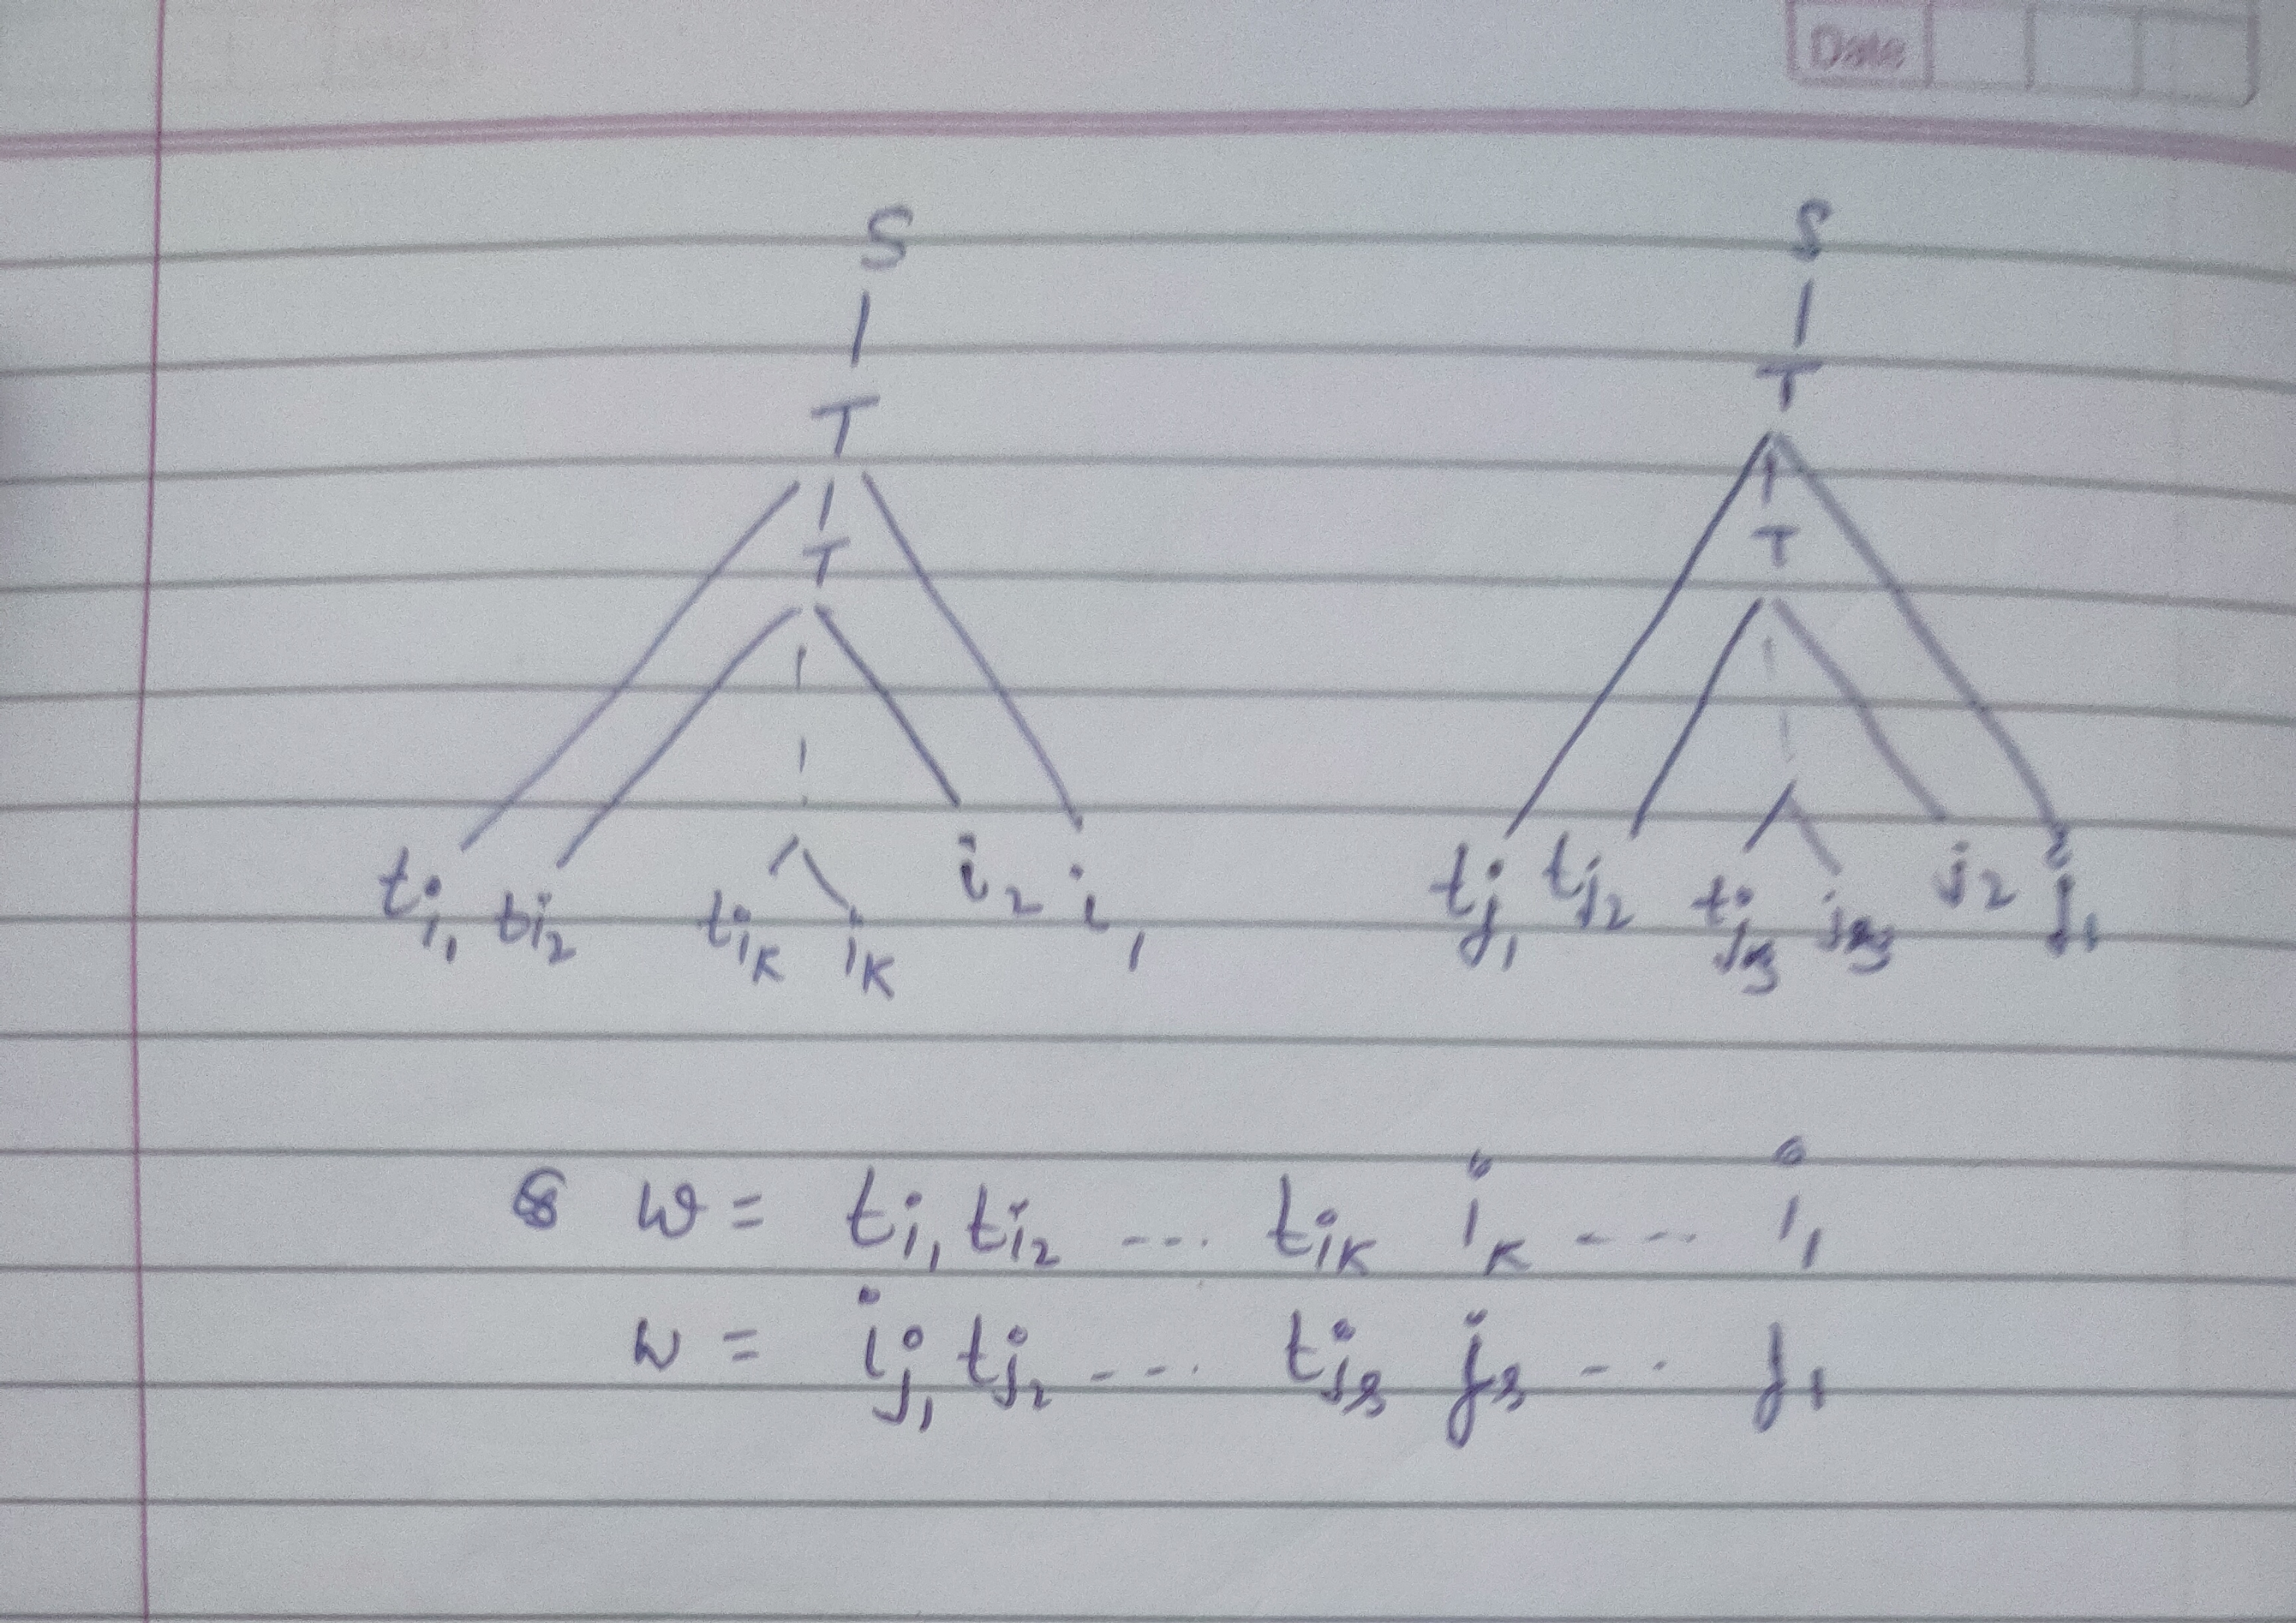
\includegraphics[width=6cm]{1.jpg}
        \caption{Case 1}
    \end{figure}

    Considering $s' = uxz$ i.e. i = 0\\
    For s' to be in A, its should be divided into 3 halves = w't'd' of equal length such that first and third are reverse.\\ 
    Since, we have removed characters from w only, w' will have all the characters of w left after removal of v,y and also some 1's 
    from t for it to have same length as other subparts of equal length (see fig 1).\\
    Hence, $1 \in w'$, but $d' \subset w^R = 0^n => 1 \notin d' => d' \neq w'^R$\\
    Hence, $s' \notin A$\\
    
    \item \textbf{Case 2:} $vxy \subseteq b $ \\

    \begin{figure}[H]
        \centering
        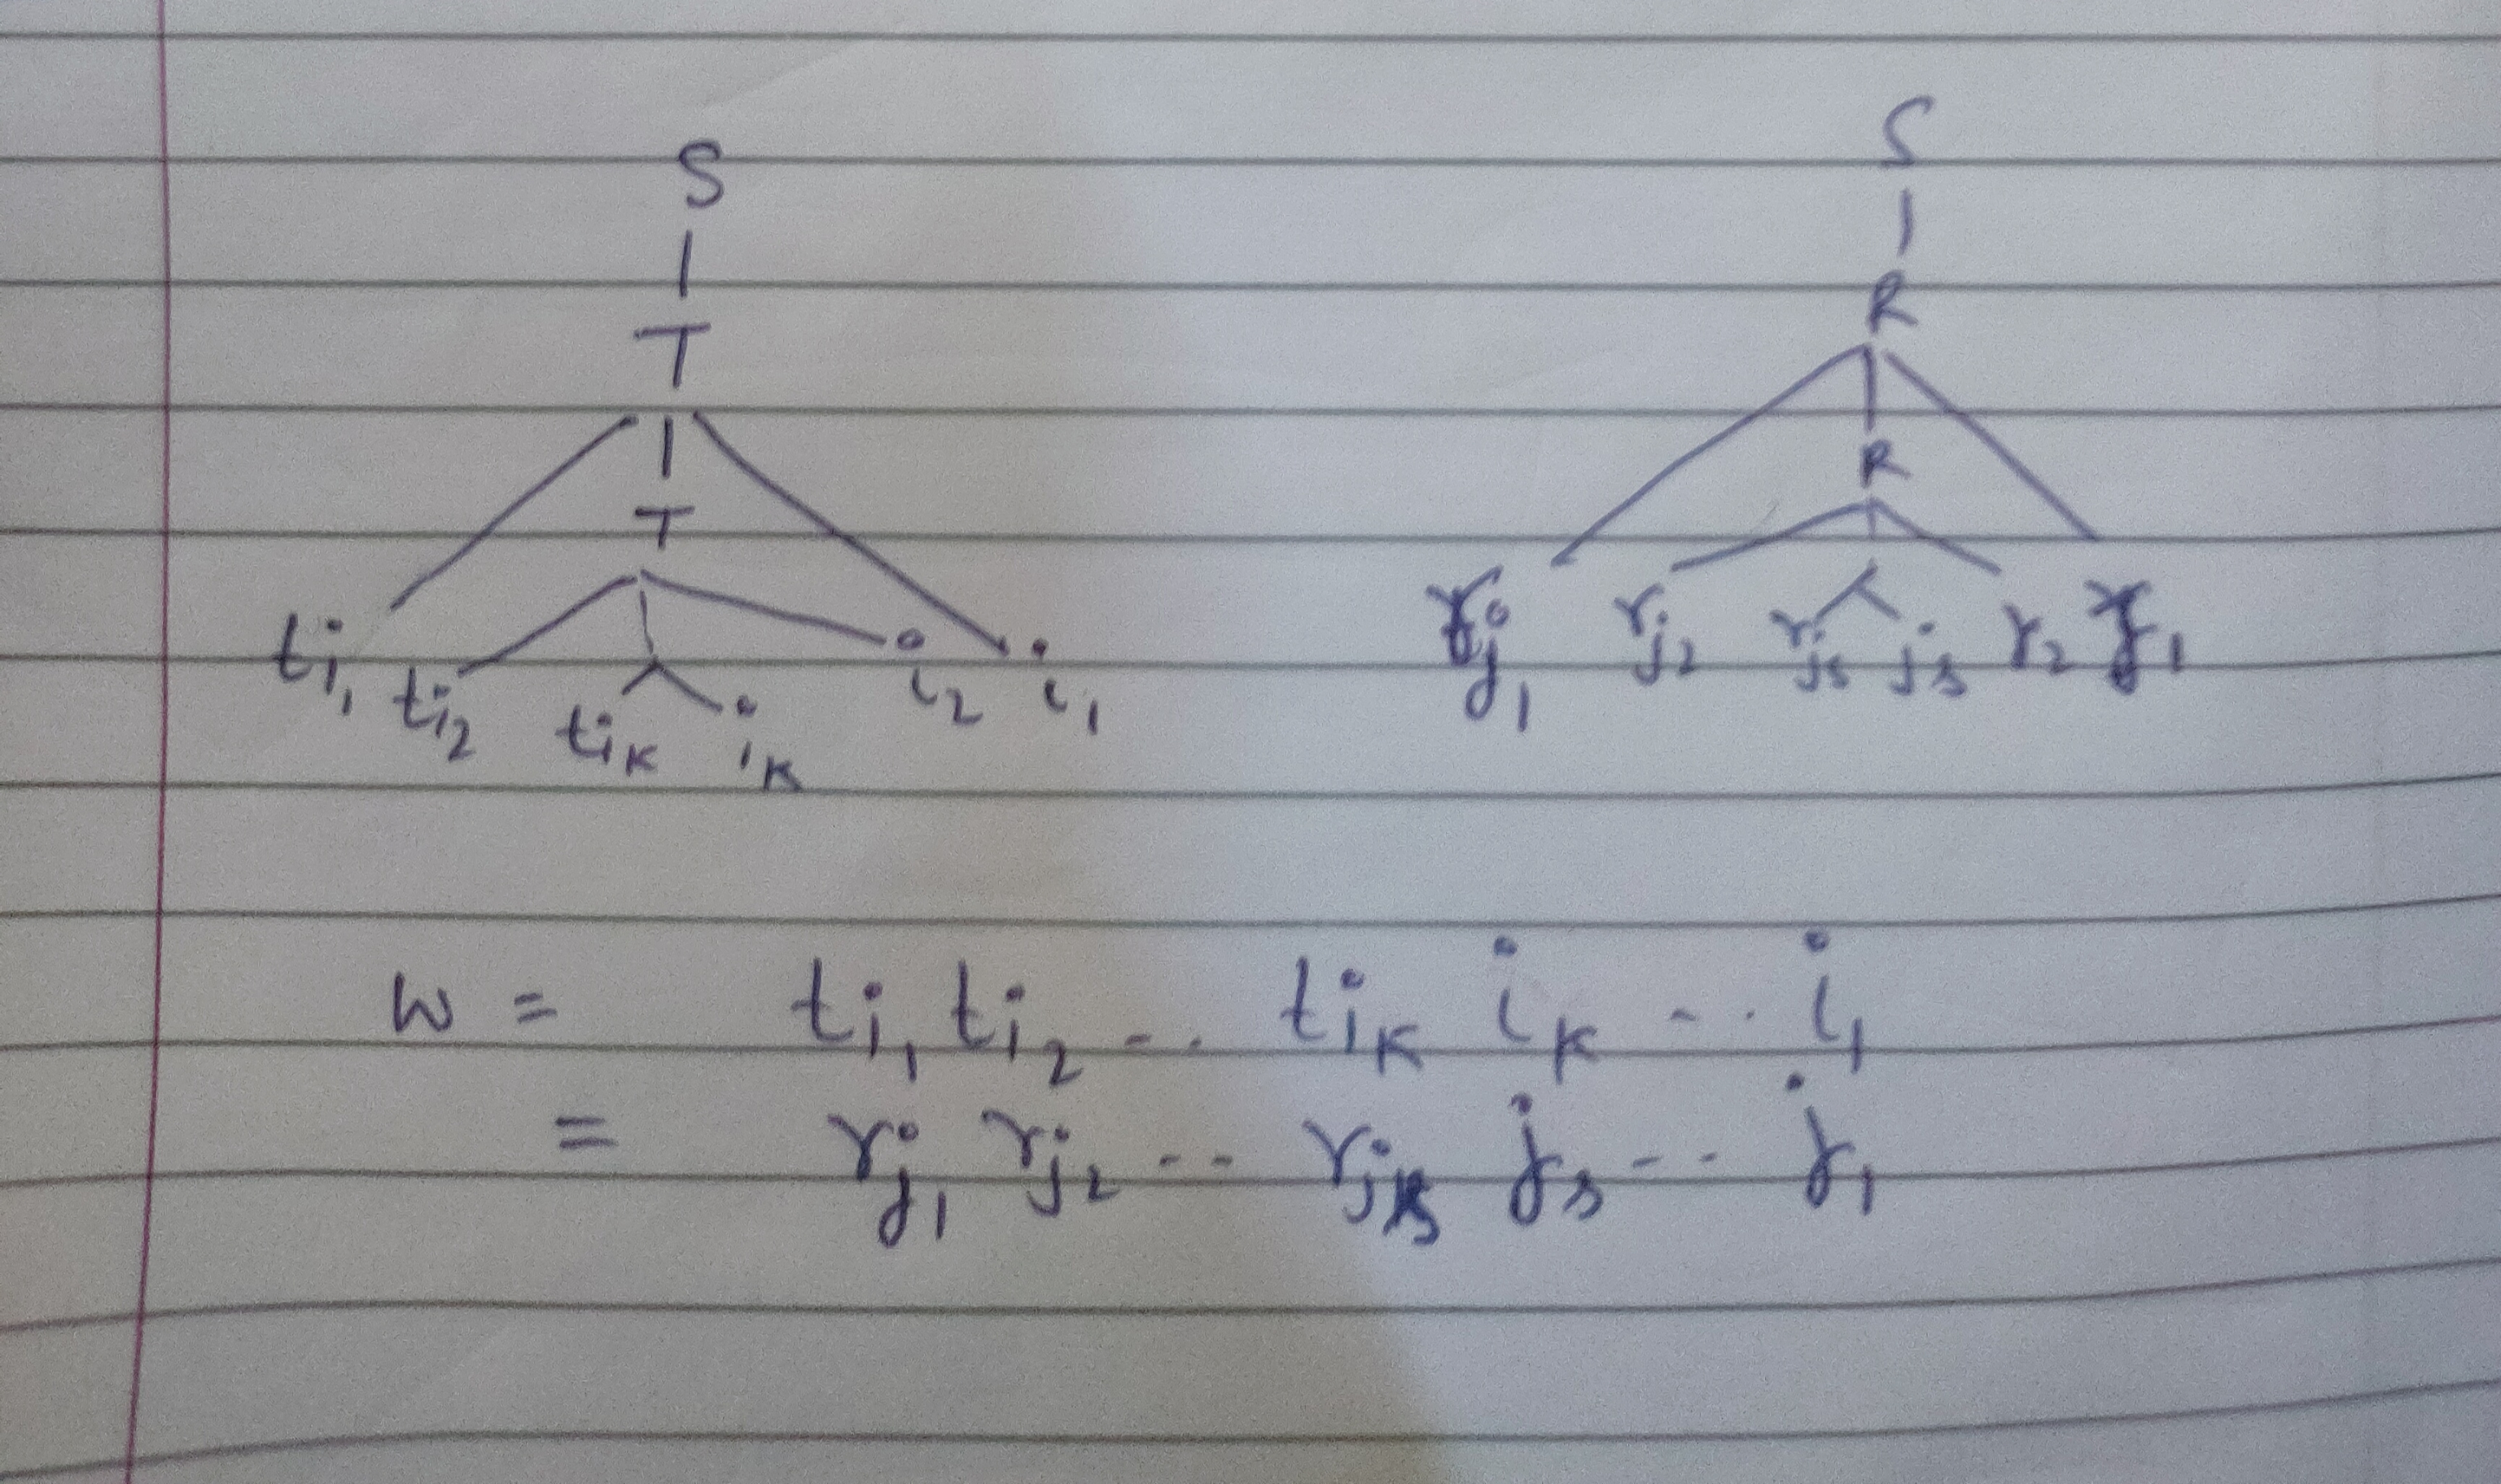
\includegraphics[width=6cm]{2.jpg}
        \caption{Case 2}
    \end{figure}

    Considering $s' = uv^2xy^2z$ i.e. i = 2\\
    Let, $|s| = l, |s'| = l', l' < l$\\
    $|w| = \frac{l}{3} < \frac{l'}{3}$\\
    $=> w \subset w' => w' $ will overflow towards t $=> 1 \in w'$\\
    But, $d' \subset w^R $ (after pumping ) that only has 0 (see fig 2)\\
    $=> d' \neq w'^R$\\
    Hence, $s' \notin A$\\

    \item \textbf{Case 3:} $vxy \bigcap a \neq \phi$\\
    
    \begin{enumerate}
        \item $w \bigcup vxy = \phi$\\
        Considering $s' = uv^2xy^2z$ i.e. i = 2\\
        This case is similar to case 2, as length of string is increased but w remains unchanged, hence w'[1:n] = w = $0^n$ and w'[n+1] = 1.
        But $(n+1)^{th}$ of d' from last = last bit of t = 0.
        $=> d' \neq w'^R$\\
        Hence, $s' \notin A$\\

        \item $w \bigcup vxy \neq \phi$\\
        Considering $s' = uxz$ i.e. i = 0\\
        This case is similar to case 1, as length of string is decreased (all from w). Hence, $1 \in w'$, but $1 \notin d'$ (from case 1) $ => d' \neq w'^R$\\
        Hence, $s' \notin A$\\
    \end{enumerate}
\end{enumerate}

Hence A is not CFL.


\pagebreak


\section{Question 6}
\textbf{Prove the following stronger version of pumping lemma for CFLs: 
If $A$ is a CFL, then there is a number $k$ where if $s$ is any string in $A$ of length at least $k$ then $s$ may be divided into five pieces $s = uvxyz$, satisfying the conditions:
\begin{enumerate}
    \item for each $i\geq 0$, $uv^ixy^iz \in A$
    \item $v \neq \varepsilon$, and $y \neq \varepsilon$, and
    \item $|vxy| \leq k$.
\end{enumerate}}

The given lemma differs from standard pumping lemma at point 2 only, so let's start the proof in a similar way to that of pumping lemma.\\
Let G = GFG for CFL A \\
b = maximum number of non terminals in the right side of any production rule.\\
$=> $ in parse tree each node will have at most b childs.\\
$=> $ a parse tree of height h corresponds to string of length at most $b^h$\\
$=> $ if $|s| \geq b^h +1$ then height of its parse tree is at least $h+1$\\

Now, set pumping length $p = b^{4|v| + 1}$, where $|V| = $ no of non terminals.\\
$\forall s : |s| \geq p = b^{4|v| + 1}$ will have height of parse tree at least $4|V| + 1$\\
Assume longest path l from start state. $|l| \geq 4|V| + 1 => $ no of non nodes in l $\geq 4|V| + 2$\\
$=> $ no of non lead nodes (non terminals) in l $\geq 4|V| + 1$\\

Now, by pegionhole principle one non terminal is repeated at least 4 times in l. Let lowest such non terminal to be R.\\
Lets name the 4 ocuurences of R to be $R_1, R_2, R_3, R_4$ from top to bottom.
Now, 2 cases are possible:\\


\begin{enumerate}
    \item \textbf{Case 1: } $\exists i,j : R_i \rightarrow_* aR_jb (a \neq \epsilon, b \neq \epsilon)$ \\ 
    Lets consider the following partition of s = uvxyz:

    \begin{figure}[H]
        \centering
        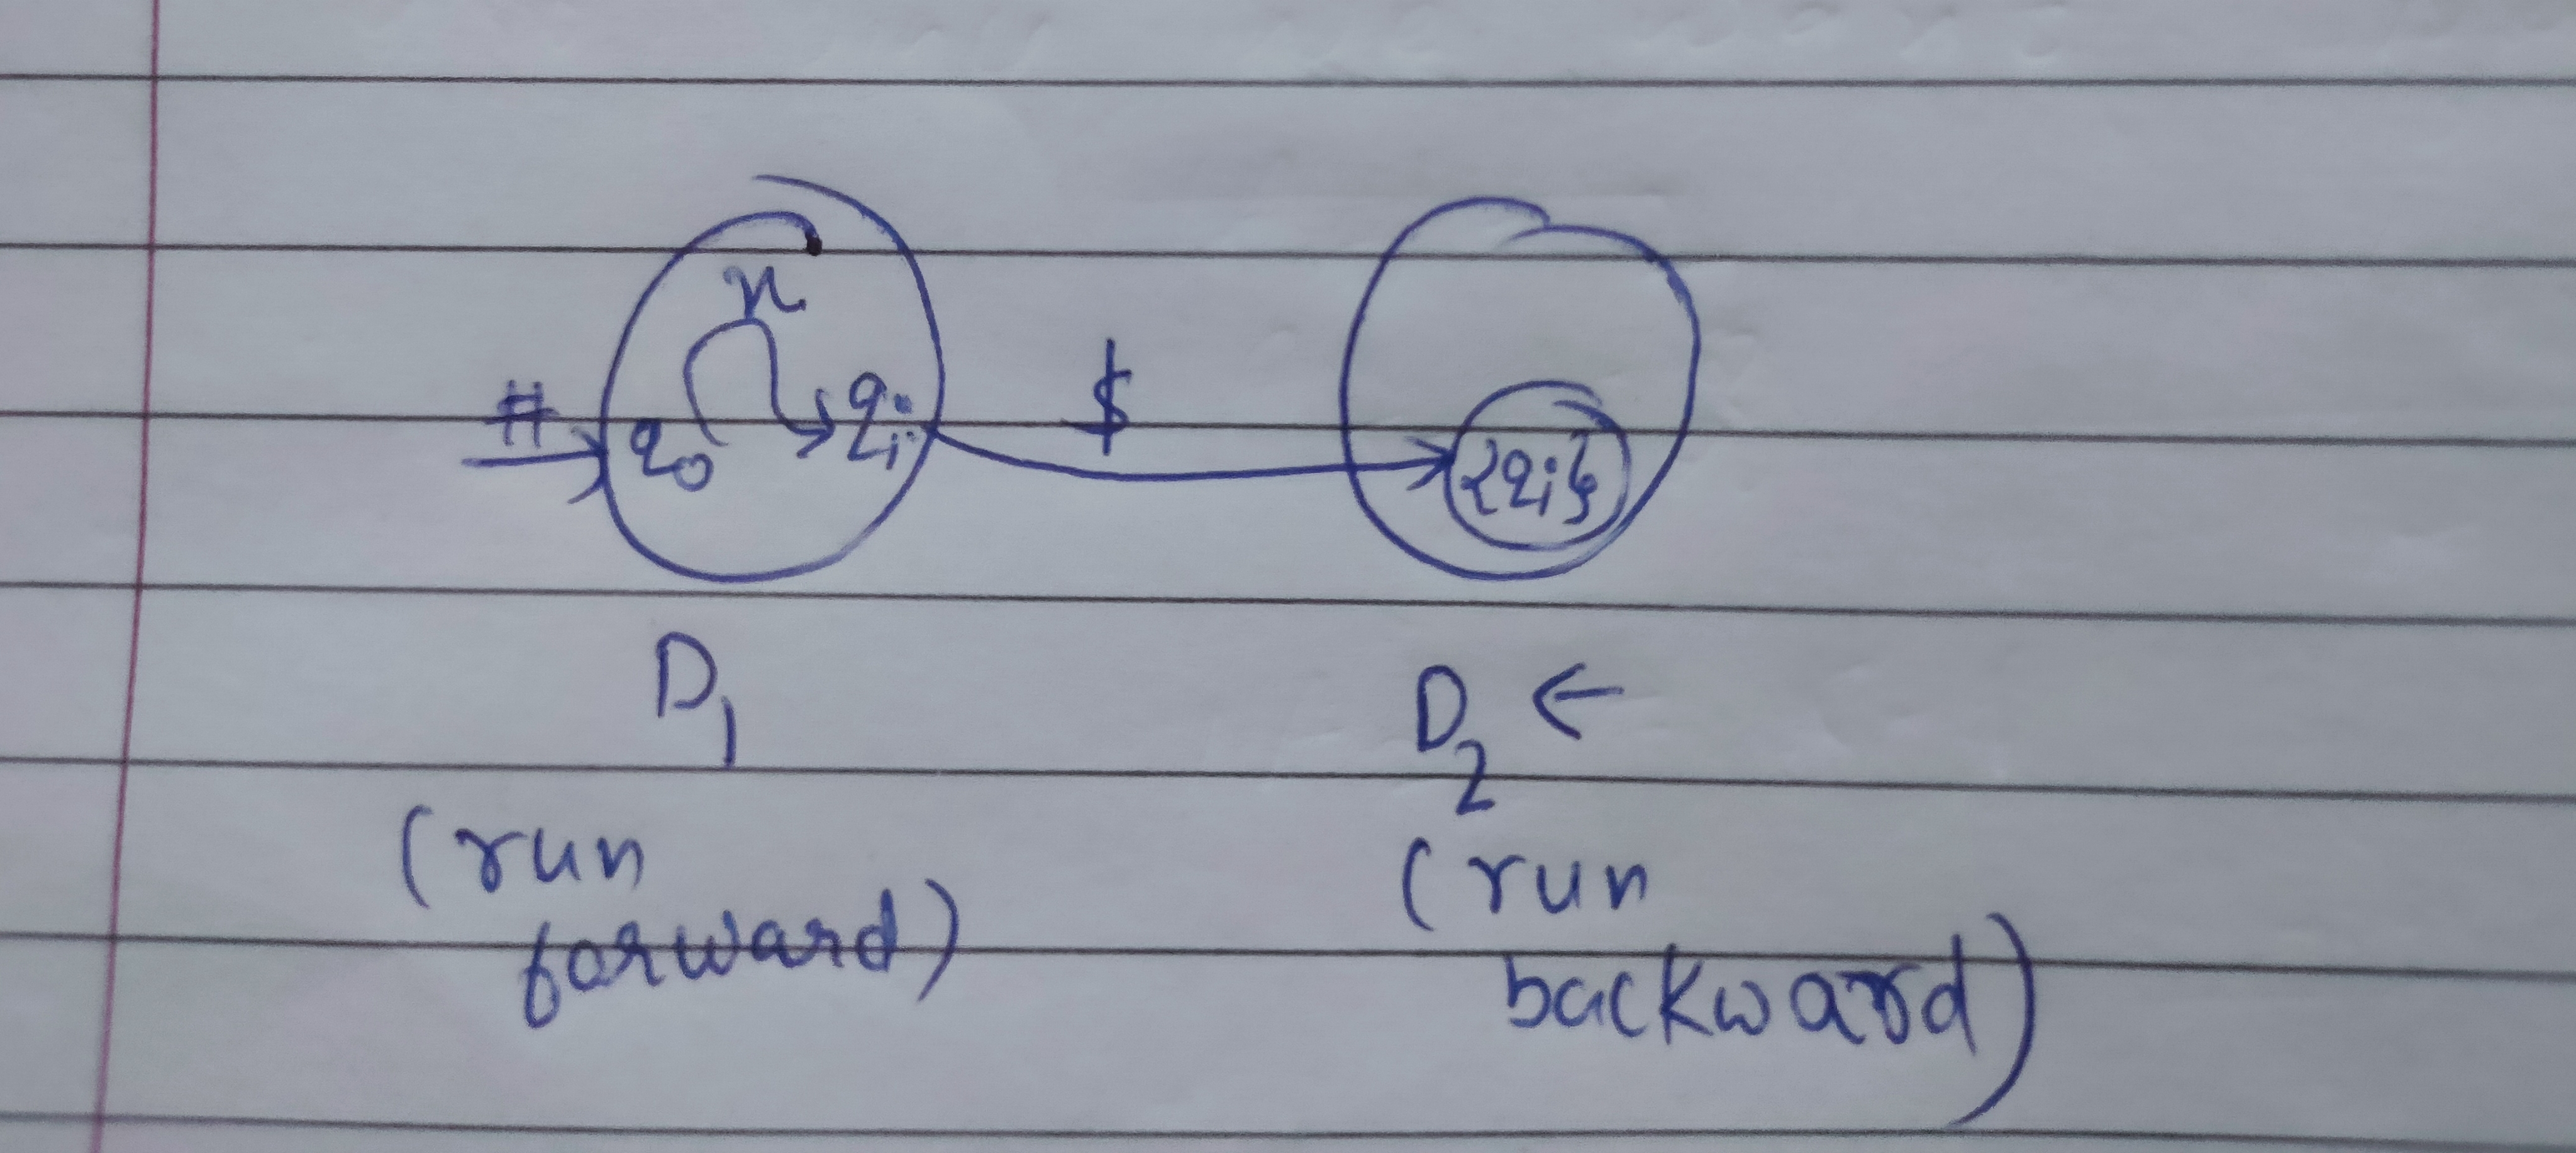
\includegraphics[width = 8cm]{3.jpg}
    \end{figure}

    i.e. a = v, b = y, subtree($R_j$) = x and remaining u and z respectively.\\
    Now, to pump down replace $R_i$ by $R_j$ giving $uxz \in A$\\
    to pump up k times, replace $R_j $ by $R_i$ k times giving $uv^kxy^kz \in A$\\
    Also, $v=a \neq \epsilon, y=b \neq \epsilon$ \\
    Moreover, since we have taken lowest repeating non terminal R, and we choose all 4 $R_i$ in the lower $4|V| + 1$ non terminals, hence string generated by 
    taking $R_1$ as root (let w) $|w| \leq b^{4|V| + 1|} = p$ and $|vxy| \leq w \leq p$\\  
    Hence done. 
    
    \item \textbf{Case 2: }$\forall i \in \{1,2,3\} : R_i \rightarrow_* R_{i+1}b (b \neq \epsilon)$\\
    Lets consider the following partition of s = uvxyz:
    \begin{figure}[H]
        \centering
        \includegraphics[width = 8cm]{4.jpg}
    \end{figure}
    To pump down replace $R_3 $ by $R_4$ and $R_1$ by $R_2$ giving $uxz \in A$\\
    To pump up k times, replace $R_4$ by $R_3$ k times, $R_2$ by $R_1$ k times giving $uv^kxy^kz \in A$.\\
    Moreover, since we have taken lowest repeating non terminal R, and we choose all 4 $R_i$ in the lower $4|V| + 1$ non terminals, hence string generated by 
    taking $R_1$ as root (let w) $|w| \leq b^{4|V| + 1|} = p$ and $|vxy| \leq w \leq p$\\  
    Hence done. 

    \item \textbf{Case 3: }$\forall i \in \{1,2,3\} : R_i \rightarrow_* aR_{i+1} (a \neq \epsilon)$\\
    This case is similar to last case just role of v is replaced by y. Performing the similar operations as that of  
    last case will give $uv^kxy^kz \in A \forall k \geq 0$\\
\end{enumerate}

These are the only 3 cases possible since both v and y cannot be $\epsilon $ simulatneously due to normal variant of pumping lemma.\\

\pagebreak


\section{Question 7}
\textbf{Give an example of a language that is not a CFL but nevertheless acts like a CFL in the pumping lemma for CFL (Recall we saw such an example in class while studying pumping lemma for regular languages). }

Consider the following languages:-\\
\begin{enumerate}
    \item $L_1 = ab^nc^nd^n$\\
        \textbf{Claim: }$L_1$ is not CFL\\
        \textbf{Proof: }Suppose $L_1$ is CFL, consider the language $L' = L_1 \bigcap b^*c^*d^* = b^nc^nd^n$\\
        Then, L' would also be regular since it is intersection of a CFL and a regular language (proved in ques 2 that intersection
        of regular langauage and CFL is CFL). But it is proved in class that L' is not a CFL. 
        Hence by contradiction $L_1$ is not CFL. 
    \item $L_2 = a^{k_1}b^{k_2}c^{k_3}d^{k_4} : k_1 \neq 1$\\
        $L_2$ is CFL because it is union of 2 regular languages : $b^*c^*d^* \bigcup a^2a^*b^*c^*d^*$ that is regular and all regular languages are CFL.
    \item $L_3 = L_1 \bigcup L_2$ \\
        $L_3$ is not a CFL as $L_3 \bigcap ab^*c^*d^* = L_1$ that is not a CFL and if $L_3$ were CFL, it should have been CFL by closure of union on CFL.
\end{enumerate}


Now, lets try to apply pumping lemma on $L_3$.\\
Let $p = 2$\\
Consider $\forall s \in L_3$\\
There are only 2 choices, either s is in $L_1$ or $L_2$ (as both have no intersection). Lets consider both of the cases seperately.\\
\begin{enumerate}
    \item $s \in L_1$\\
    Consider the partition of s = uvxyz, where $u = v = x = \epsilon, y = a, z = b^nc^nd^n (n > 0 as |s| \geq 2)$ \\
    Now, $\forall i \geq 0 : s' = uv^ixy^iz = a^ib^nc^nd^n$\\
    If i = 1 then $s'=s \in L_1 => s' \in L_3$ otherwise $s' $ is of the form  $a^{k_1}b^{k_2}c^{k_3}d^{k_4} : k_1 \neq 1$ i.e. $s' \in L_2 => S' \in L_3$\\
    $=> \forall i \geq 0 s' \in L_3$\\
    Hence $L_3$  satisfies pumping lemma.
    \item $s \in L_2$ \\
    This case is simple as $L_2$ is CFL, it should satisfy pupming lemma. Hence we are done.
\end{enumerate}
Hence provided an NCFL that satisfies pumping lemma.
\pagebreak


\end{document}
